%=======================================================================
%  Real-Time Embedded Systems 2026 — Final Assignment
%  Architecture of the Bluesky Jetstream Firehose Collector
%
%  Compile with XeLaTeX:
%      latexmk -xelatex architecture.tex
%=======================================================================
\documentclass[11pt,a4paper]{article}

\usepackage{fontspec}
\setmainfont{DejaVu Serif}
\setsansfont{DejaVu Sans}
\setmonofont{DejaVu Sans Mono}[Scale=0.82]

\usepackage[margin=1.8cm]{geometry}
\usepackage{booktabs}
\usepackage{array}
\usepackage{url}
\usepackage{graphicx}
\usepackage{float}
\usepackage{enumitem}
\usepackage{xcolor}
\usepackage{siunitx}
\usepackage{tikz}
\usetikzlibrary{arrows.meta,positioning,fit,backgrounds}
\usepackage[hidelinks]{hyperref}

\definecolor{pc}{HTML}{2E5E8C}
\definecolor{sc}{HTML}{3F7A3F}
\definecolor{lc}{HTML}{8C3F3F}
\definecolor{gc}{HTML}{5A5A5A}
\definecolor{bg}{HTML}{F2F4F7}

\newcommand{\code}[1]{\texttt{\small #1}}
\setlength{\parskip}{2pt}
\emergencystretch=1.5em

\title{\vspace{-1.6cm}\textbf{A Multithreaded Real-Time Collector for the\\ Bluesky Jetstream Firehose}\\[0.3em]
\large Architecture, Synchronisation and Verification}
\author{Embedded Systems --- Final Assignment\\[0.3em]
\small\url{https://github.com/EvangelosMoschou/Embedded_assignment}}
\date{September 2026}

\begin{document}
\maketitle
\vspace{-1.4cm}

%-----------------------------------------------------------------------
\section{System Overview}
%-----------------------------------------------------------------------

The system is a self-contained acquisition node that runs unattended for 24\,h on a
Raspberry Pi Zero W --- a \emph{single-core} ARM1176 (ARMv6, 32-bit) at 1\,GHz with
512\,MB of RAM and no real-time kernel. It subscribes to the public Bluesky Jetstream
firehose over a WebSocket (\url{wss://jetstream1.us-east.bsky.network/subscribe?wantedCollections=app.bsky.feed.post}),
classifies every incoming JSON message by its top-level \code{kind} field
(\code{commit}, \code{identity}, \code{account} or \code{info}), and appends one line
of telemetry per second. Traffic is non-uniform --- 39.5 messages per second on average
with peaks above 340 --- so three activities with incompatible timing requirements must
coexist: ingestion is bursty and must never block, classification is
throughput-oriented, and telemetry is strictly periodic. They are placed on separate
threads and decoupled by a bounded buffer, so a delay in one cannot propagate into the
others; the goals are \emph{low jitter}, \emph{zero data loss} and \emph{bounded memory}
rather than hard-deadline guarantees.

%-----------------------------------------------------------------------
\section{Architecture}
%-----------------------------------------------------------------------

\begin{figure}[H]
\centering
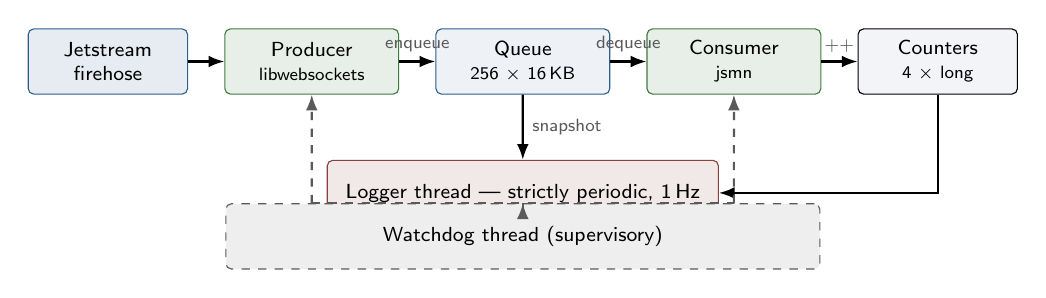
\begin{tikzpicture}[
    scale=0.92, transform shape,
    node distance=5mm and 5mm,
    box/.style={draw, rounded corners=2pt, minimum height=9mm,
                align=center, font=\footnotesize\sffamily, fill=bg, inner sep=3pt},
    net/.style={box, fill=pc!12, draw=pc, minimum width=22mm},
    work/.style={box, fill=sc!12, draw=sc, minimum width=24mm},
    qbox/.style={box, fill=pc!8, draw=pc, minimum width=24mm},
    logb/.style={box, fill=lc!12, draw=lc},
    wd/.style={box, fill=gc!10, draw=gc, dashed},
    ar/.style={-{Latex[length=2mm]}, thick},
    lab/.style={font=\scriptsize\sffamily, text=gc}
]
\node[net]  (net)  {Jetstream\\firehose};
\node[work, right=of net]  (prod) {Producer\\\scriptsize libwebsockets};
\node[qbox, right=of prod] (q)    {Queue\\\scriptsize 256 $\times$ 16\,KB};
\node[work, right=of q]    (cons) {Consumer\\\scriptsize jsmn};
\node[box,  right=of cons, minimum width=22mm]
                           (ctr)  {Counters\\\scriptsize 4 $\times$ long};
\node[logb, below=9mm of q, minimum width=54mm]
             (log)  {Logger thread --- strictly periodic, 1\,Hz};
\node[wd, below=15mm of q, minimum width=82mm]
             (wd)   {Watchdog thread (supervisory)};

\draw[ar] (net) -- (prod);
\draw[ar] (prod) -- node[lab, above]{enqueue} (q);
\draw[ar] (q)    -- node[lab, above]{dequeue} (cons);
\draw[ar] (cons) -- node[lab, above]{++} (ctr);
\draw[ar] (q.south)   -- node[lab, right, pos=0.5]{snapshot} (log.north);
\draw[ar] (ctr.south) |- (log.east);

\coordinate (busL) at (prod.south |- wd.north);
\coordinate (busR) at (cons.south |- wd.north);
\draw[dashed, thick, draw=gc] (busL) -- (busR);
\draw[ar, dashed, draw=gc] (wd.north) -- (wd.north |- busL);
\draw[ar, dashed, draw=gc] (busL) -- (prod.south);
\draw[ar, dashed, draw=gc] (busR) -- (cons.south);
\end{tikzpicture}
\caption{Data flow. The producer and the logger touch the queue; the consumer and
the logger touch the counters; the logger is the only thread performing I/O; the
watchdog only observes.}
\end{figure}

\textbf{Producer (asynchronous, network-facing).} It owns a single libwebsockets
client context and runs the event loop \code{lws\_service(ctx, 50)}, performing
no downstream processing: a complete message is enqueued, the consumer is
signalled, and control returns to the network immediately, so socket buffers are
drained as fast as possible. Two details are essential. First,
\emph{reassembly}: libwebsockets delivers anything larger than its receive buffer
as several callbacks, so fragments are accumulated in a 16\,KB staging buffer and
published only when \code{lws\_is\_final\_fragment()} reports the end of the
frame --- otherwise one message would be parsed as several invalid ones. Second,
\emph{bounded insertion}: if the queue is full the frame is dropped and counted
rather than blocking the network thread, because blocking there would lose data
at a layer the application cannot observe. On failure the producer reconnects
with exponential backoff (1, 2, 4, \dots, 60\,s), reset after any connection that
lasted longer than a minute.

\textbf{Consumer (event-driven, no I/O).} It sleeps on the queue's condition
variable and, for each message, releases the slot, parses the JSON with
\textbf{jsmn} --- a zero-allocation tokeniser (256 tokens, \code{JSMN\_PARENT\_LINKS})
whose cost is independent of message size --- and increments the corresponding
counter under its own mutex. Per the specification this thread performs no screen
output and no file I/O. Classification is made robust by falling back to the
tokens parsed so far whenever the parser reports an error, which happens when a
frame exceeds the 16\,KB slot; since \code{kind} appears near the beginning of a
Jetstream message, such frames are still counted correctly instead of discarded.

\textbf{Logger (strictly periodic).} It is the only thread with side effects on
storage and the component whose timing is measured. It fires exactly once per
second from \code{clock\_nanosleep(CLOCK\_MONOTONIC, TIMER\_ABSTIME, \&next, NULL)},
where \code{next} is advanced by one second from the \emph{previous ideal
deadline} rather than from the actual wake-up. Each activation it locks the
counter mutex briefly to read and reset the four counters, samples the queue
occupancy, computes CPU utilisation from \code{/proc/stat}, and appends a
\code{CLOCK\_REALTIME} timestamp. The absolute-deadline scheme is what prevents
drift from accumulating: a late wake-up shortens the next interval instead of
shifting every subsequent sample, so drift is zero by construction and any
residual deviation of the \code{Seconds} column is attributable to the wall
clock, not the scheduler. Sampling once per second also bounds the observer
effect on the other threads to one short critical section per second, regardless
of the message rate.

\textbf{Watchdog (supervisory).} A fourth, non-essential thread observes the
liveness of the three workers through atomic heartbeats; if a worker reports no
progress for 5\,s the process exits with a non-zero status, which the
\code{systemd} unit (\code{Restart=always}) turns into a fresh process. It also
emits the \code{WATCHDOG=1} notification required by \code{WatchdogSec}, and
takes part in no data path --- it only ever reads shared state.

%-----------------------------------------------------------------------
\section{Synchronisation and Race Conditions}
%-----------------------------------------------------------------------

Two mutexes protect the two shared structures, and no lock is ever held across a
blocking call:

\begin{center}\small
\begin{tabular}{@{}llll@{}}
\toprule
\textbf{Shared state} & \textbf{Protected by} & \textbf{Written by} & \textbf{Read by}\\
\midrule
Queue (head, tail, count, peak) & \code{fq.mut}       & producer & consumer, logger\\
Message counters                & \code{counters\_mut} & consumer & logger\\
\bottomrule
\end{tabular}
\end{center}

The queue is a classical bounded-buffer of \textbf{256 slots of 16\,KB each},
statically allocated (4\,MB), with \emph{two} condition variables: the producer
waits on \code{notFull} and the consumer on \code{notEmpty}. Deadlock is avoided
because each condition variable is signalled only while holding the queue mutex,
and because the consumer releases the slot \emph{before} parsing, so the slow
part never blocks the producer. Three further details resolve specific races:
(i)~the consumer's wait is a \emph{one-second timed wait} that refreshes its
heartbeat on each timeout --- a plain \code{pthread\_cond\_wait()} would make an
idle consumer, for instance during a 60\,s reconnect backoff, indistinguishable
from a dead one; (ii)~the termination handler performs a single atomic store and
nothing else, since \code{pthread\_cond\_broadcast()} is not async-signal-safe,
and the other threads notice the flag within one second; (iii)~the shared
heartbeats and the shutdown flag are C11 atomics of \textbf{4-byte} width, a
deliberate choice --- on ARMv6 8-byte atomics are not lock-free and would require
linking against \code{libatomic} (Section~\ref{sec:verify}).

%-----------------------------------------------------------------------
\section{Log File}
%-----------------------------------------------------------------------

Telemetry is appended to a single file, \code{metrics\_log.txt}, with exactly the
prescribed eight comma-separated fields --- \code{Seconds} and \code{Nanoseconds}
from \code{clock\_gettime(CLOCK\_REALTIME)}, the four per-second message counters
(reset after each sample), the queue occupancy at the instant of logging, and the
\code{/proc/stat} CPU utilisation over the preceding second. The header is written
only when the file is created, so a restart continues the same dataset instead of
injecting a header line into the middle of it.

%-----------------------------------------------------------------------
\section{Off-Target Verification}
\label{sec:verify}
%-----------------------------------------------------------------------

Because the Pi was intended to run unattended for 24\,h, the code was first exercised
entirely off-target: a \textbf{mock firehose server} with an exactly known message
distribution checks the logged counters against ground truth, three \textbf{sanitiser
builds} verify bounds, leaks and locking, an \textbf{ARMv6 cross-compile} probe
confirms that the target build keeps the lock-free guarantee, and a \textbf{leak probe}
repeats the time-driven operations 86\,400 times. It was not merely confirmatory: it
found four defects that would have corrupted the dataset, including misclassification
of fragmented messages and false watchdog termination during network outages. After
correction the suite reports exact counter agreement and no memory growth.

%-----------------------------------------------------------------------
\section{Measured Results}
%-----------------------------------------------------------------------

Measured on the deployed system over a continuous 24-hour window
(20 September 2026, 00:00:00--23:59:59 local time):

\begin{center}\small
\begin{tabular}{@{}lrl@{}}
\toprule
\textbf{Quantity} & \textbf{Value} & \textbf{Notes}\\
\midrule
Samples logged        & 86\,394 of 86\,400 & 99.993\,\% coverage\\
Message rate          & 39.5\,Hz mean, 343\,Hz peak & peak-to-mean ${\approx}8.7\times$\\
Jitter, median        & \SI{104}{\micro\second} & 95th pct.\ \SI{362}{\micro\second}\\
Jitter, 99th pct.     & \SI{845}{\micro\second} & worst case \SI{18.1}{\milli\second}\\
Queue occupancy       & 13.7\,\% peak & 35 of 256 slots; 0 frames dropped\\
CPU, whole process    & 7.8\,\% mean & of one core\\
Resident memory       & 12.5\,MB & of which 4\,MB pre-allocated queue\\
\bottomrule
\end{tabular}
\end{center}

\begin{figure}[H]\centering
\includegraphics[width=0.80\textwidth]{figs/overview.png}
\caption{The three required plots over the full 24 hours.
\textbf{(a)}~\emph{Jitter}: deviation from the absolute deadline (grey, $\geq 0$ by
construction) and the signed deviation of each one-second period from the ideal (dark).
\textbf{(b)}~\emph{Load and buffer}: message rate vs.\ buffer occupancy.
\textbf{(c)}~\emph{CPU}: message rate vs.\ CPU utilisation.}
\end{figure}

Two observations follow. The timing cost is dominated by TLS and WebSocket framing in
the network thread, not by the work of the assignment; and the queue occupancy is best
read as \emph{headroom}, since the peak scales with the message rate while never
approaching saturation --- which is why the drop counter stayed at zero.

%-----------------------------------------------------------------------
\section{Long-Run Behaviour and Network Resilience}
%-----------------------------------------------------------------------

\textbf{Zero loss.} The drop counter stayed at zero for the whole window: every frame
the network delivered was enqueued and classified. Frames larger than the 16\,KB slot
(well below 0.02\,\% of the total) were still classified correctly and are counted
separately as truncated.

\textbf{One recovered stall.} At 14:43:38 the producer stopped renewing its heartbeat
while consumer and logger continued normally (the watchdog logged \code{p=7 c=1 l=1},
and the logger's jitter stayed near \SI{100}{\micro\second}). No disconnection, storage
error, kernel message or thermal event accompanied it, so the blocker lay inside the
network library with the connection established. The watchdog terminated the process
after 5\,s, \code{systemd} restarted it 5.5\,s later, and the socket returned within a
further second: \textbf{6 seconds out of 86\,400} (0.007\,\%). At 01:28:17 the log shows
an \emph{identical} seven-second interval with no messages and \emph{no} restart, since
the producer was alive and only the server was quiet --- so the criterion is not
``absence of data'' but ``absence of progress by the thread''.

\textbf{Flapping is absorbed.} 64 disconnections and 62 reconnections occurred over
about thirty hours, in bursts of up to 21 in one hour. Each produced an automatic
reconnection with exponential backoff; none restarted the process, lost a classified
message, or produced a segmentation fault.

\textbf{Memory is bounded.} Resident memory settled at ${\sim}12.5$\,MB, with growth
decaying from 1900\,kB per hour initially to ${\sim}150$\,kB per hour after eight hours ---
the signature of a statically allocated working set reaching its high-water mark, not a
leak, corroborated by \code{malloc\_stats()} (1.43\,MB reserved, 1.08\,MB in use).

\end{document}
